% MERGE - Data
%%%%%%%%%%%%%%%%%%%%%%%%%%%%%%%%%%%%%%%%%%%%%

% FR
%Cette dernière partie permet de faire le liant entre le modèle de transport calculé dans le premier paragraphe et l'application développée dans le second paragraphe. L'objectif final étant de visualiser les informations des habitudes de transport à vélo dans la ville de Hyvinkää au travers un navigateur web. Pour ce faire, nous nous appuierons sur les notions expliqués dans les paragraphes précédents : le modèle de transport aquis et calculé, l'application développée et configurée.

% EN
This last part allows for the binder between the transport model calculated in the first paragraph and the application developed in the second paragraph. The ultimate goal is to view information bicycle transportation habits in the city of Hyvinkää through a web browser. 

To do this, we will build on the concepts explained in the preceding paragraphs: the transport model acquired and calculated, the application developed and configured.

%%%%%%%%%%%%%%%%%%%%%%%%%%%%%%%%%%%%%%%%%%%%%%%%%%%%%%%%%%%%%%%%%%%%%%%%%
% FR
%\section{Services REST}

% EN
\section{REST Services}

% FR
% Pour que l'application puisse interagir avec le serveur, nous avons besoin de services REST expliqué dans le chapitre 2. Le script Python exécuté en Deamon sur le serveur propose des services REST. Chaque service est appellé par une requête HTTP depuis l'application puis retourne un JSON contenant les données demandées.

% EN

For the application to interact with the server, we need REST services described in chapter 2. The Python script running on the server in Deamon offers REST services. Each service is called by an HTTP request from the application and returns a JSON containing the requested data.

This service is based on python micro-framework Flask. Backend environment you can see in Fig. \ref{img.asas}
\begin{figure}
\centering
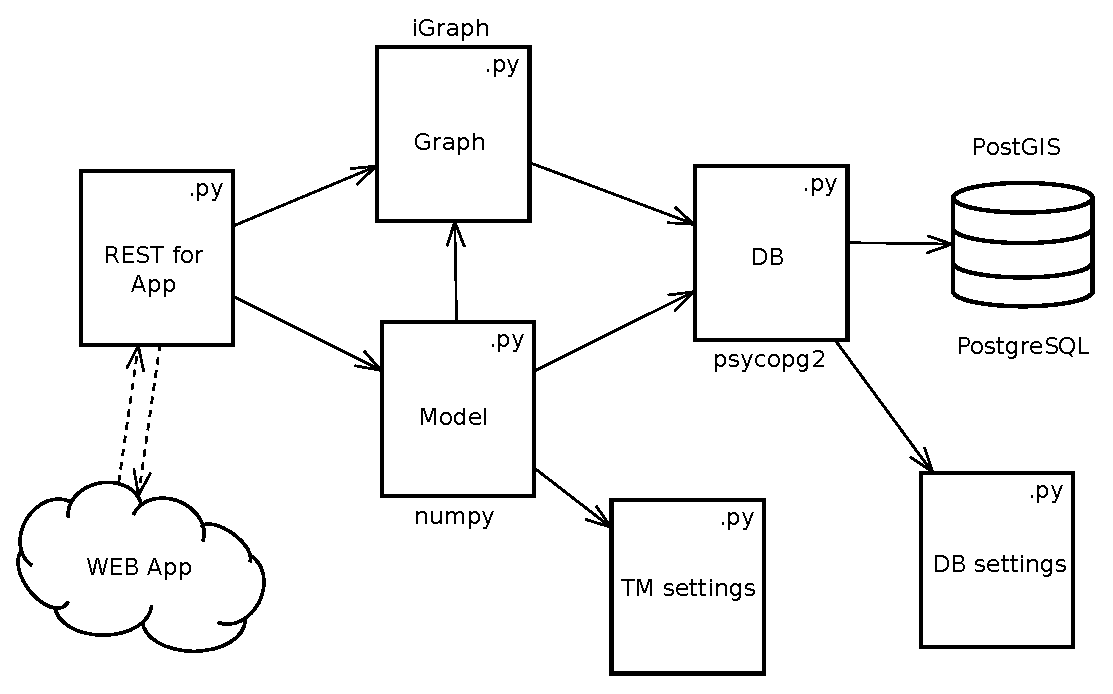
\includegraphics[width=15cm]{img/c01-transp-model/backend.eps}
\caption{Backend (REST)}
\label{img.asas}
\end{figure}

% FR
% La suite de ce paragraphe décrit chacun des services nécessaires et utilisés par l'application et explique les formats de JSON retournés.

% EN
The rest of this section describes each of the necessary services and used by the application and explains returned JSON formats.

\begin{description}

  \item[/api] \hfill \\ 
    Return an HTML list of all services on the REST API, with an example. \\
    \begin{lstlisting}[language=html]
<h2>Api info for TraMap</h2>
<ul>
  <li><b>/api/interests</b> - return type for tables (don't need any parameters)</li>
  <li><b>/api/ssp</b> - return Shortest path from A to B e.g
    <a href="api/ssp?lon1=24.87078&lat1=60.61663&lon2=24.85747&lat2=60.63003">
        api/ssp?lon1=24.87078&lat1=60.61663&lon2=24.85747&lat2=60.63003
    </a></li>
  <li><b>/api/compute_traffic</b> - start compute traffic (return info about start compute)</li>
  <li><b>/api/compute_traffic_progress</b> - progress for compute traffic</li>
<ul>
    \end{lstlisting}   
  \item[/api/interests] \hfill \\ 
    Return a JSON object with all the interests point by table. \\
    \begin{lstlisting}[language=javascript]
  {
    "status" : "ok",
    "result" : [
      {
        "table" : "roads",
        "interests" : [
          "motorway",
          "footway",
          "cycleway",
          "..."
        ]
      },{...}
    ]
  }
    \end{lstlisting} 
    
  \item[/api/ssp] \hfill \\ 
  
    Return a JSON object with the geometry shortest path, 
    time (in seconds) and distance (in meters) \\
    \begin{lstlisting}[language=javascript]
  {
    "status":"ok",
    "result":{
      "distance":1941.2000656999999,
      "features":[
        {
          "type":"LineString",
          "coordinates":[
          [
            24.8714912,
            60.6171716
          ],
          [
            24.8706363,
            60.6168433
          ],
          [
            24.870383,
            60.6167319
            ]
          ]
        },
        {...}
      ]
    }
  }
    \end{lstlisting}
    
  \item[/api/compute\_traffic] \hfill \\ 
  Recompute traffic take a lot of time, so REST must be asynchronous. In our approach we made two service. First service start compute and second return progress.  
    If you call this service, server start recomputing traffic and return information about start of recompute. \\
    \begin{lstlisting}[language=javascript]
{
"status": "ok",
"result": "calculation began"
}
    \end{lstlisting}
    
  \item[/api/compute\_traffic\_progress] \hfill \\ 
    This service is for view progress of recomputing traffic. Service return progress in \%.\\
    \begin{lstlisting}[language=javascript]
{
"status": "ok",
 "result": {
 			"progress": 34,
 			"isrun": true
 		   }
}
    \end{lstlisting}
  
\end{description}

% \begin{figure}[h]
%   \centering
%   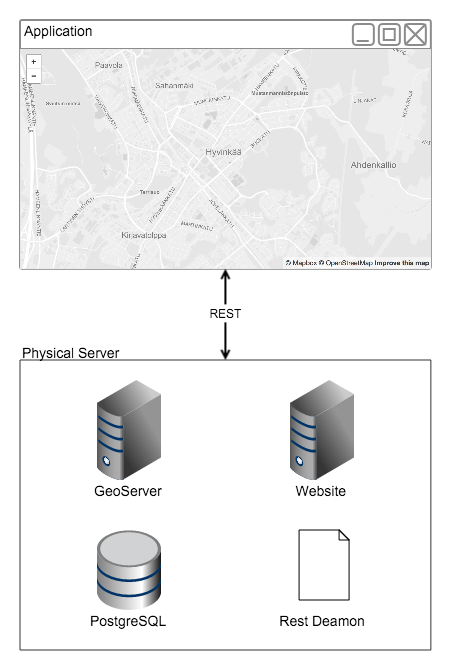
\includegraphics[width=8cm]{img/c02-application/png/app-server-interact.png}
%   \caption{Interaction between the application and the server}
% \end{figure}


